\begin{tikzpicture}\tikzstyle{every node}=[font=\small]
  \node[inner sep=0pt] (iphone) at (7,0) {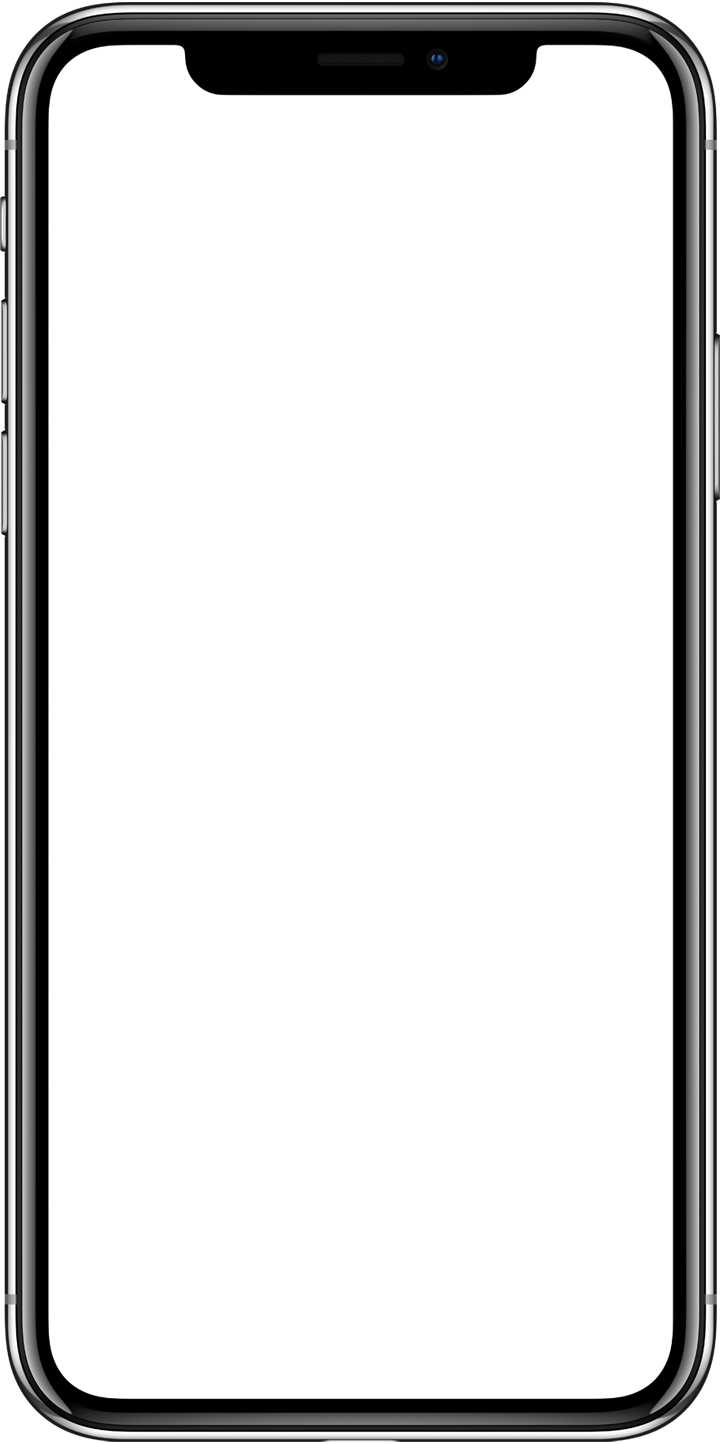
\includegraphics[width=.35\textwidth]{Figures/iphone.png}};
  \node[graduate, minimum size=1.5cm] (user) at (0,0) {Utilisateur};
  \node[draw, ellipse, align=center] (connect) at (7,3) {Se connecter \\ Se déconnecter};
  \node[draw, ellipse, align=center] (schedule) at (7,1) {Consulter les \\ horaires des cours};
  \node[draw, ellipse, align=center] (notif) at (7,-1) {Recevoir \\ des notifications};
  \node[draw, ellipse, align=center] (param) at (7,-3) {Changer \\ les paramètres de \\ notifications};
\draw (user.east) -- (connect.west);
\draw (user.east) -- (schedule.west);
\draw (user.east) -- (notif.west);
\draw (user.east) -- (param.west);
\end{tikzpicture}